\hypertarget{software-manipulasi-audio}{%
\section{Software Manipulasi Audio}\label{software-manipulasi-audio}}

\hypertarget{audacity}{%
\subsection{Audacity}\label{audacity}}

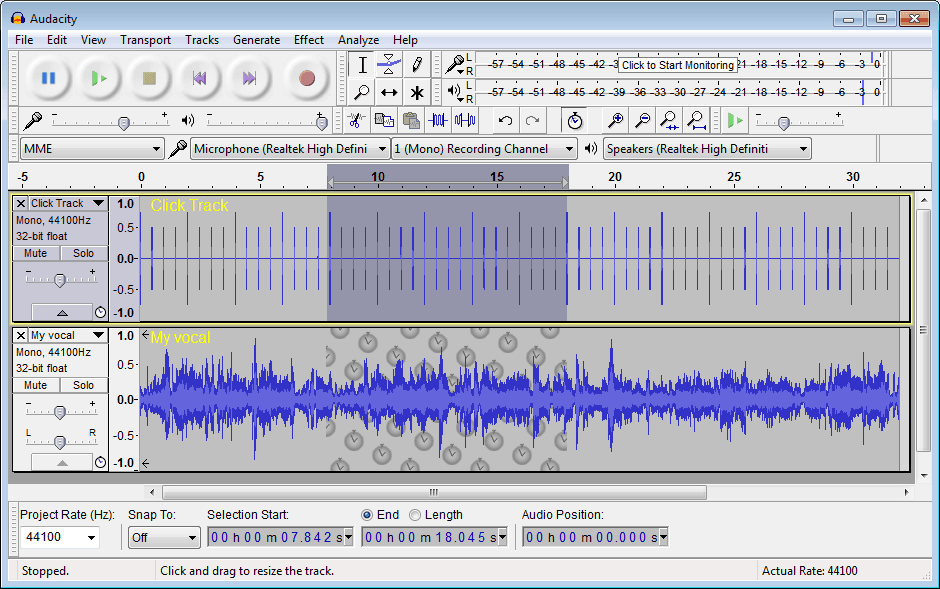
\includegraphics{images/audacity.png} Audacity adalah aplikasi
manipulasi audio gratis dan \emph{open source} (satu-satunya di list
ini) untuk sistem operasi Windows, Mac, dan Linux.

Audacity memiliki beberapa fitur dasar untuk memanipulasi audio,
seperti:

\begin{itemize}
\tightlist
\item
  Audio Recording
\item
  Multitrack Recording and Editing
\item
  Scrubbing
\item
  MIDI Playback
\item
  Penggunaan plugin VST (hanya terbatas untuk VST Effect, bukan MIDI)
\item
  Analisa Spektrum Audio
\item
  dsb
\end{itemize}

Audacity unggul di harga dan fleksibilitasnya. Sebagai satu-satunya
aplikasi yang gratis di list ini serta UI yang mudah digunakan, Audacity
banyak dipakai oleh banyak Audio Engineer pemula dan juga pembawa
podcast di seluruh dunia. Hanya saja, kekurangan Audacity dapat dilihat
dari kurangnya support untuk driver ASIO, Perekaman MIDI, dan juga
tampilan UI-nya yang terbilang \emph{jadul} dan tidak profesional.

\hypertarget{adobe-audition}{%
\subsection{Adobe Audition}\label{adobe-audition}}

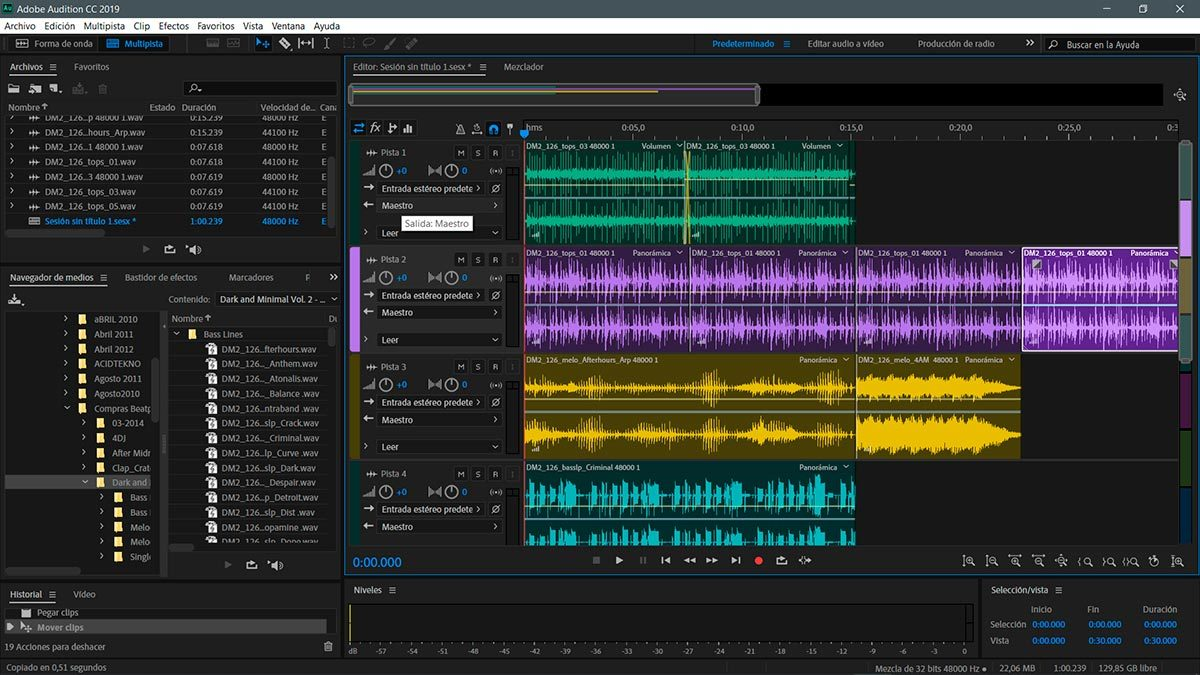
\includegraphics{images/audition.jpg} Adobe Audition merupakan salah
satu dari keluarga aplikasi Adobe Creative Cloud yang dimiliki oleh
Adobe. Audition dapat dijalankan baik di Windows maupun Mac.

Beberapa fitur unggulan Adobe Audition antara lain,

\begin{itemize}
\tightlist
\item
  Analisis Frekuensi Audio secara langsung
\item
  Dynamic Link
\item
  Project Manager
\item
  Mengedit audio dalam video
\end{itemize}

Adobe Audition banyak dipakai oleh audio engineer di dunia karena
Audition memiliki integrasi yang sangat kuat dengan aplikasi Adobe
lainnya, seperti Premiere Pro, After Effects, dll. Sayangnya, Adobe
Audition memiliki masalah yang kurang lebih sama seperti software
lainnya, yaitu tidak stabil (sering crash dan hang). Selain itu,
Audition juga dipatok dengan harga yang cukup mahal dan menggunakan
pembayaran dengan cara berlangganan, sehingga tidak semua orang dapat
membelinya.

\hypertarget{ableton-live}{%
\subsection{Ableton Live}\label{ableton-live}}

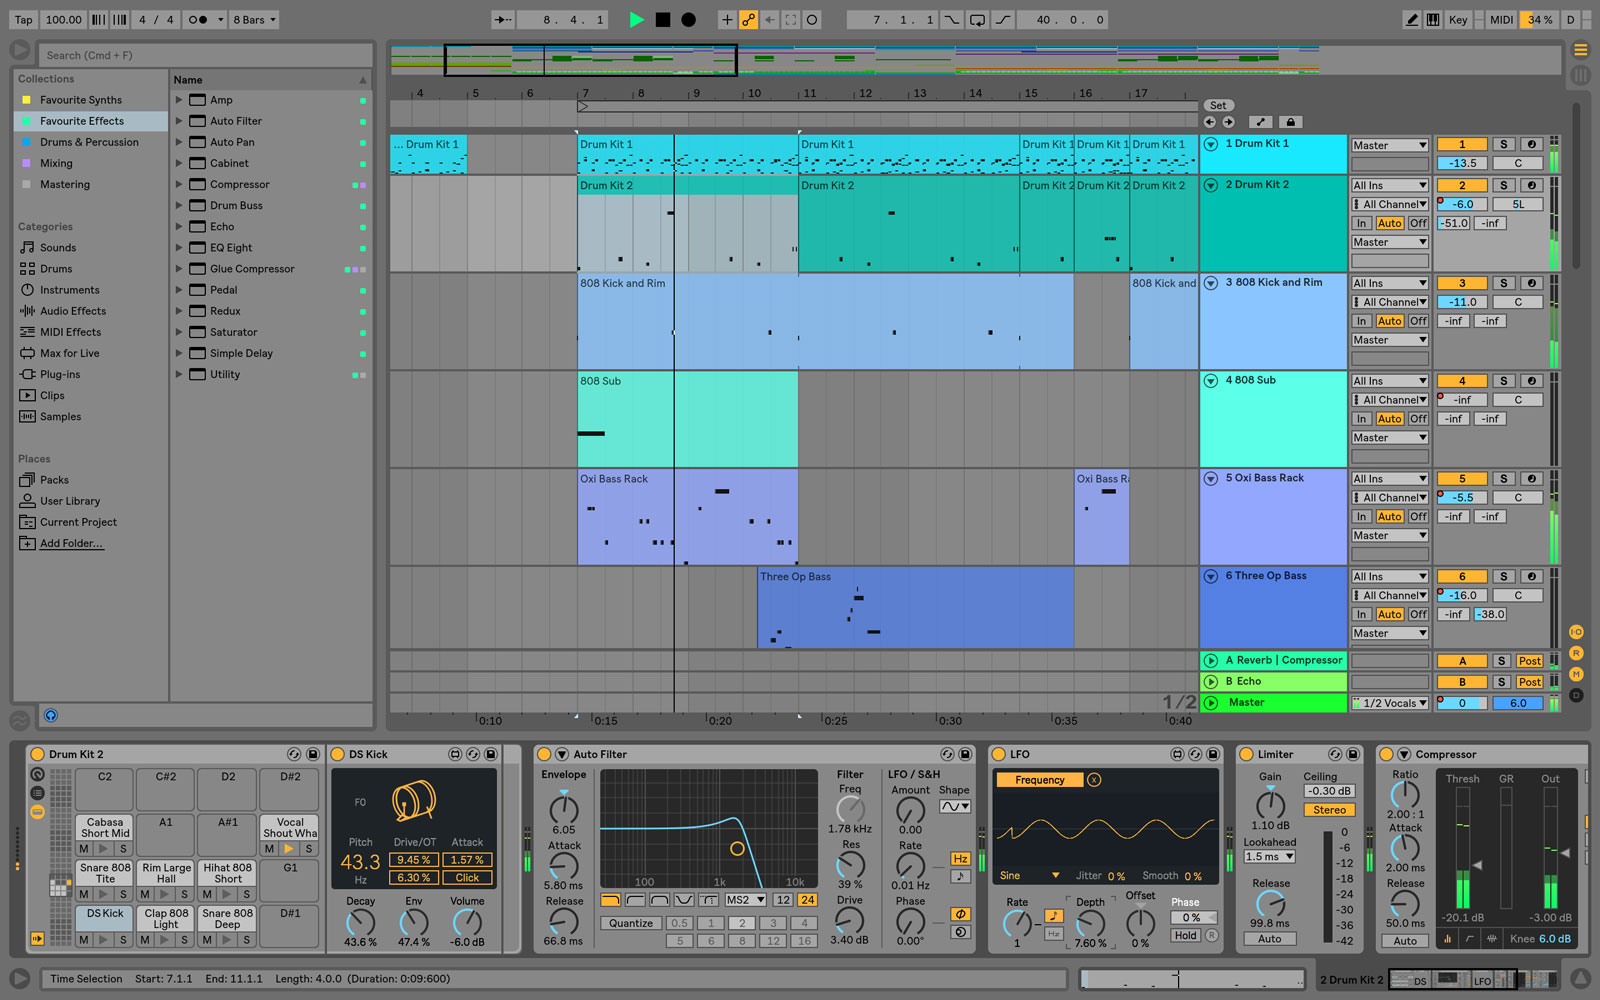
\includegraphics{images/ableton.jpg} Ableton Live adalah aplikasi
Digital Audio Workstation yang dapat dijalankan di Windows dan Mac.
Aplikasi DAW seperti ini biasanya ditargetkan untuk kalangan produser
musik untuk membuat musik, tapi banyak juga yang memakai DAW sebagai
aplikasi recording dan manipulasi audio biasa.

Fitur unggulan Ableton Live antara lain,

\begin{itemize}
\tightlist
\item
  UI yang sederhana
\item
  Kemampuan untuk menggunakan Loop dan Sample
\item
  Banyaknya \emph{built-in effects} yang disediakan
\end{itemize}

Ableton Live lebih ditargetkan kepada musisi dan produser hip-hop dan
electronic karena kemampuan looping dan samplingnya yang lebih kuat
dibanding aplikasi lainnya. Hanya saja, harga dari Ableton Live
tergolong sangat mahal meskipun \emph{one-time purchase}. Selain itu,
meskipun Ableton memiliki UI yang sederhana, tapi tampilannya dapat
mengintimidasi pengguna baru dan orang awam.

\hypertarget{logic-pro}{%
\subsection{Logic Pro}\label{logic-pro}}

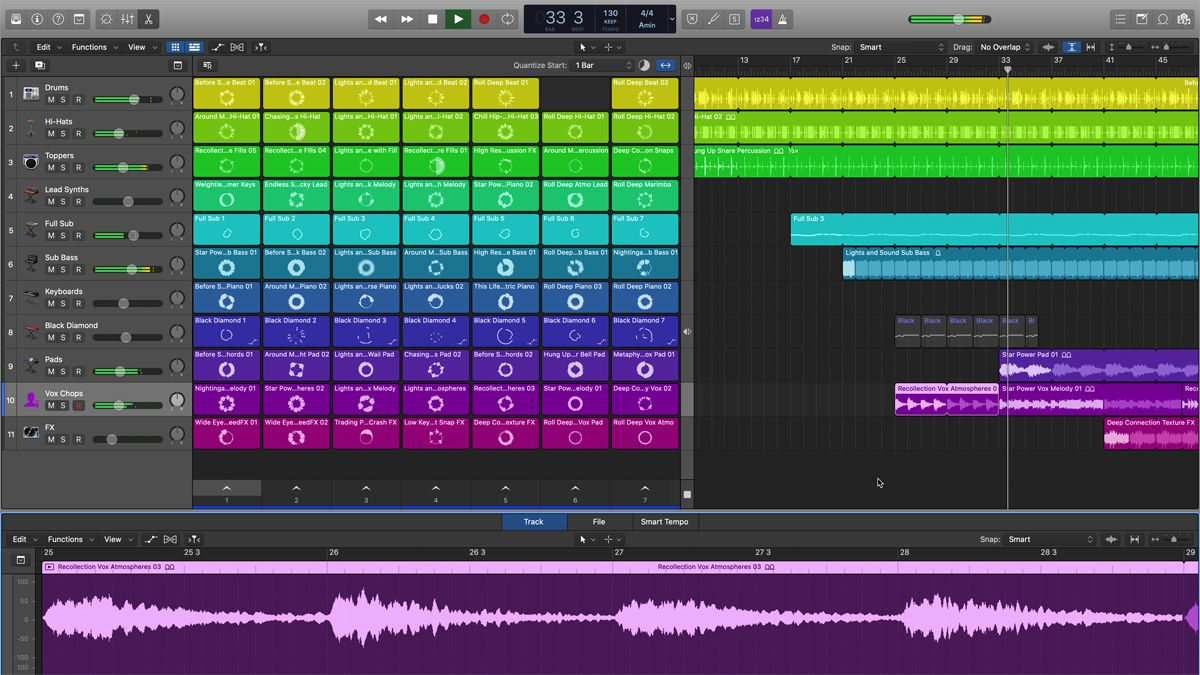
\includegraphics{images/logic.jpg} Logic Pro adalah aplikasi DAW dari
Apple yang hanya bisa digunakan di Mac saja. Aplikasi ini merupakan
salah satu standar industri (selain Pro Tools) yang banyak dipakai di
studio terkenal di seluruh dunia.

Beberapa fitur unggulan Logic Pro antara lain,

\begin{itemize}
\tightlist
\item
  Performa yang lebih baik
\item
  Tampilan UI yang menyerupai peralatan Analog tapi tetap mempertahankan
  modernitas
\item
  Memiliki fitur audio recording lebih lengkap ketimbang yang lainnya
\end{itemize}

Karena dibuat dan didesain oleh Apple, maka tentu performa yang
dihasilkan dari aplikasi ini tentu sangat responsif ketika digunakan.
Tapi \emph{trade-off}nya adalah Logic hanya bisa digunakan pada sistem
Mac saja. Logic juga memiliki kemampuan analog/audio recording yang
lebih baik ketimbang kompetitor lainnya tapi hal itu juga ditukar dengan
kemampuan recording MIDI dsb yang kurang.

\hypertarget{fl-studio}{%
\subsection{FL Studio}\label{fl-studio}}

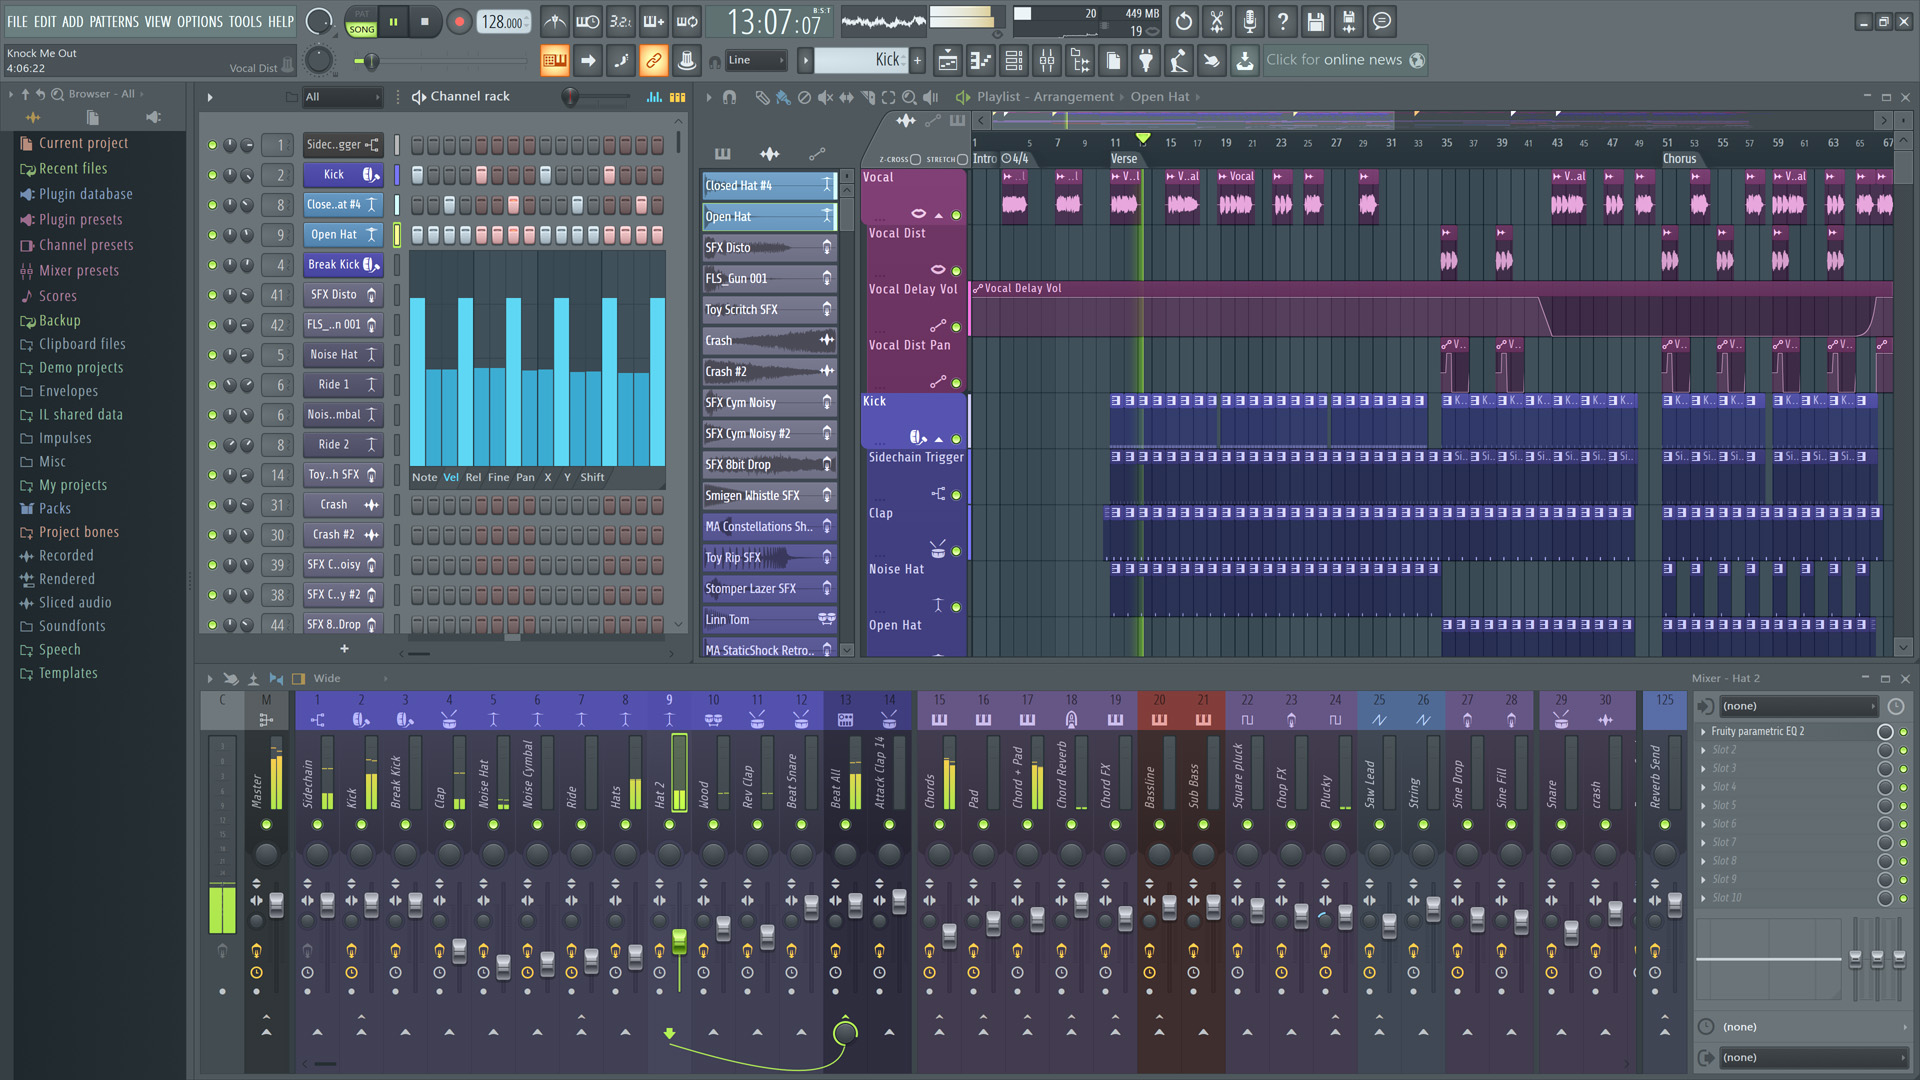
\includegraphics{images/flstudio.jpg} FL Studio merupakan aplikasi DAW
yang dikembangkan oleh Image-line dan dapat digunakan di Windows dan
Mac. Aplikasi ini terkenal di kalangan produser Indonesia karena
banyaknya tutorial di Youtube dan juga tampilan yang mudah digunakan.

Fitur unggulan dari FL Studio antara lain,

\begin{itemize}
\tightlist
\item
  UI yang sederhana dan modern
\item
  Tersedia banyak tutorial dan pelatihan di internet
\item
  Sequencer yang intuitif
\end{itemize}

FL Studio memiliki UI yang sangat mudah digunakan sehingga tidak heran
banyak orang di Indonesia yang menggunakan aplikasi ini. Selain itu,
\emph{built-in effects} yang cukup banyak serta mudah digunakan
merupakan salah satu poin pendukung aplikasi ini. Tapi FL Studio
memiliki workflow yang menurut saya sedikit \emph{clunky} dan juga
kemampuan mixing yang menurut saya kurang fleksibel. Tapi mungkin banyak
orang yang sudah terbiasa dan juga lebih tertarik terhadap workflow dan
UI aplikasi ini. Selain itu, FL Studio juga memberikan \emph{Lifetime
Free Upgrade} tidak seperti aplikasi kompetitor lainnya (kecuali
Audacity dan Audition)

\hypertarget{reaper}{%
\subsection{Reaper}\label{reaper}}

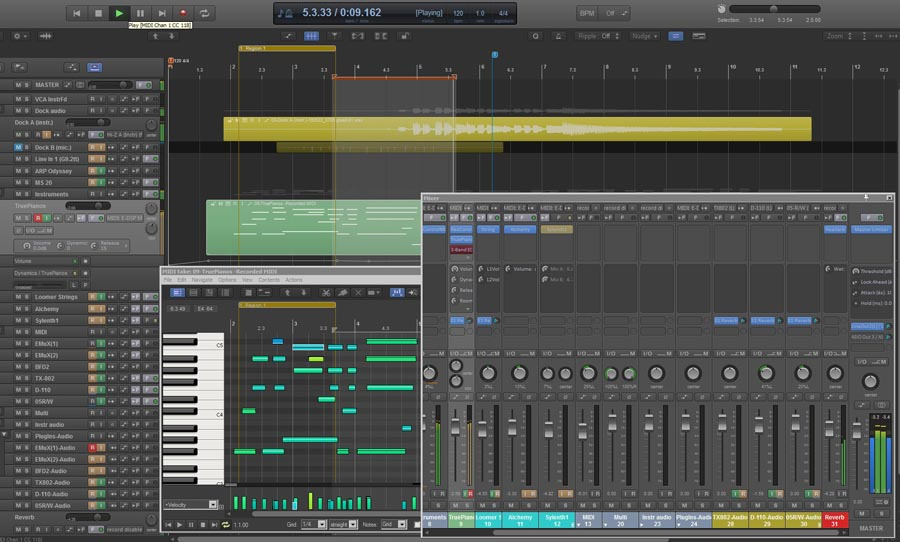
\includegraphics{images/reaper.jpg} Reaper sangat kuat dan kaya fitur
juga relatif lebih terjangkau. Sebagai permulaan, Reaper hadir dengan
dukungan untuk beberapa trek, dan memiliki dukungan~multichannel~yang
luar biasa dengan 64 saluran di setiap trek.

Reaper juga memiliki kemampuan untuk merekam~audio~langsung
ke~mono,~stereo~atau bahkan file~audio~multikanal, bersama dengan
kemampuan untuk merekam ke beberapa~disk~pada saat yang sama untuk
redundansi data. Hanya saja,~user interface~dari Reaper tidak sebagus
Adobe Audition dan Reaper agak sulit dipakai oleh pemula.

\hypertarget{presonus-studio-one}{%
\subsection{Presonus Studio One}\label{presonus-studio-one}}

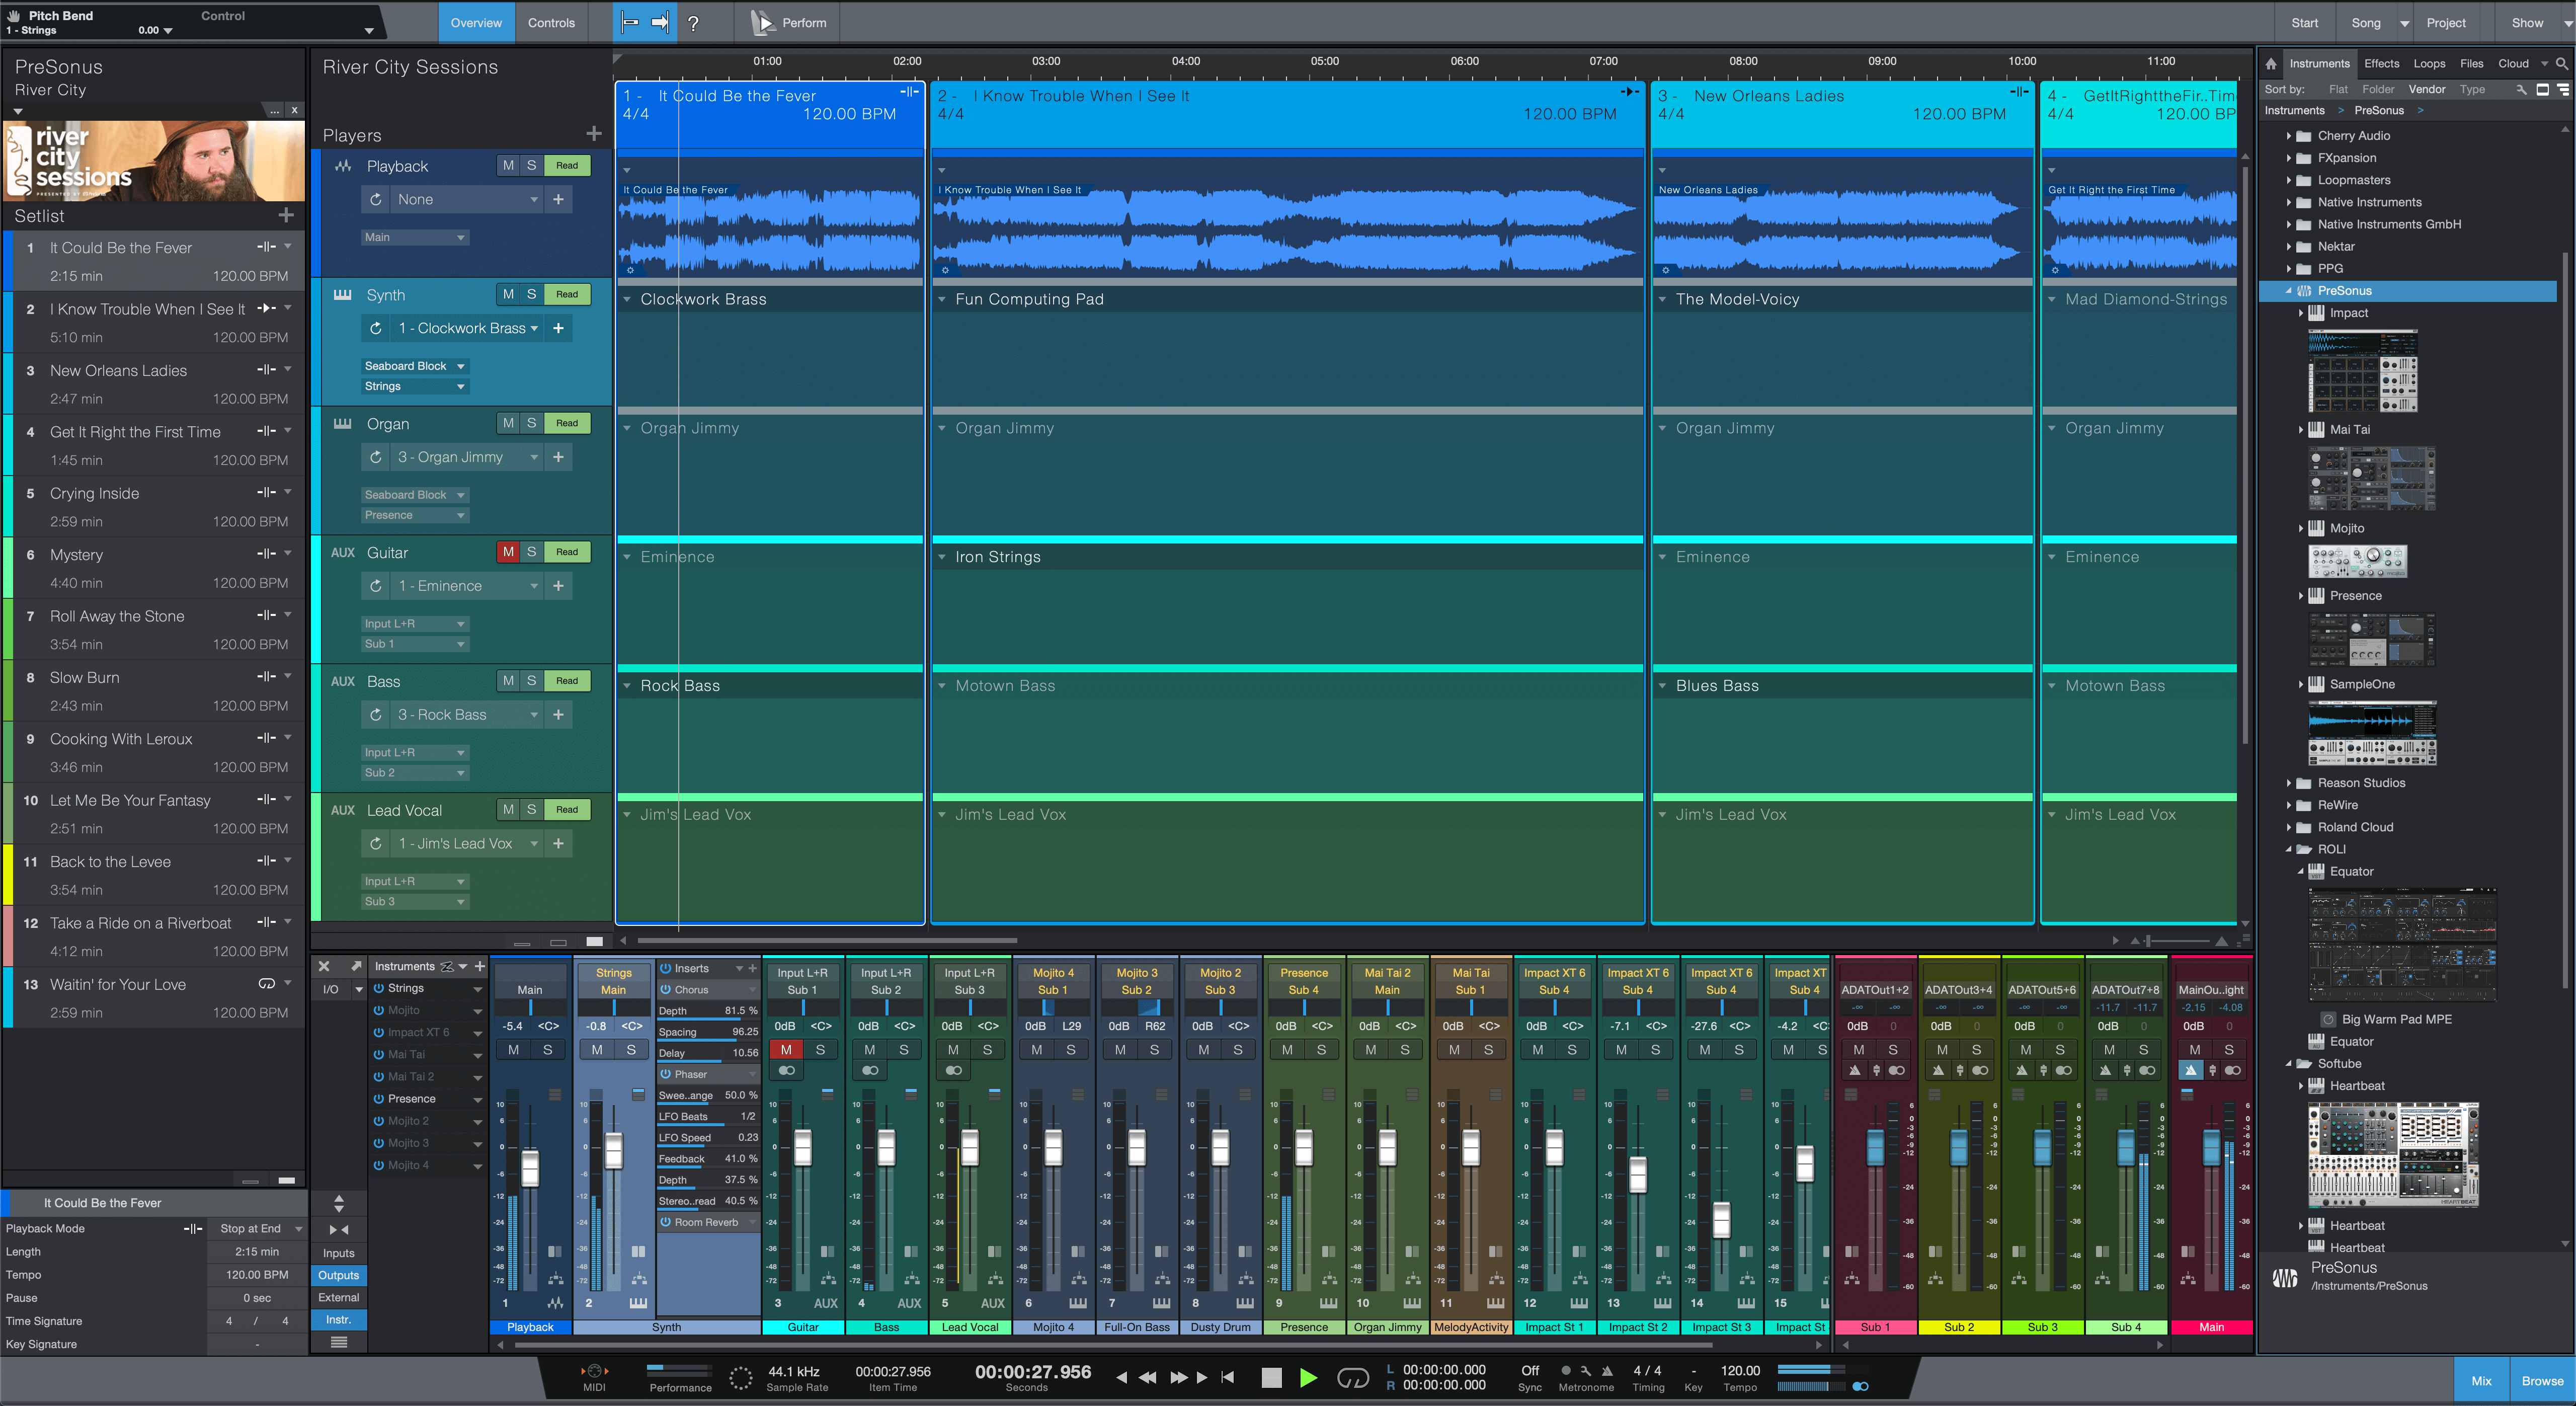
\includegraphics{images/studioone.png} Presonus Studio One 4 adalah DAW
serbaguna yang hadir dengan banyak fitur keren dan berguna. Ada dukungan
untuk beberapa trek, dan dengan fitur Chord Track Studio One, sehingga
bisa dengan mudah membuat prototipe cepat dari suatu lagu dan
mendapatkan gagasan tentang seperti apa lagu itu terdengar.

\emph{Chord Track} membawa fitur seperti modulasi kunci, substitusi akor
dan lainnya untuk membuat protoyping lebih mudah. Studio One dapat
secara otomatis mengidentifikasi chord dari track~audiomu. Namun untuk
pemula software ini kurang cocok karena \emph{learning curve} yang cukup
tinggi.

\hypertarget{hindenburg-pro}{%
\subsection{Hindenburg Pro}\label{hindenburg-pro}}

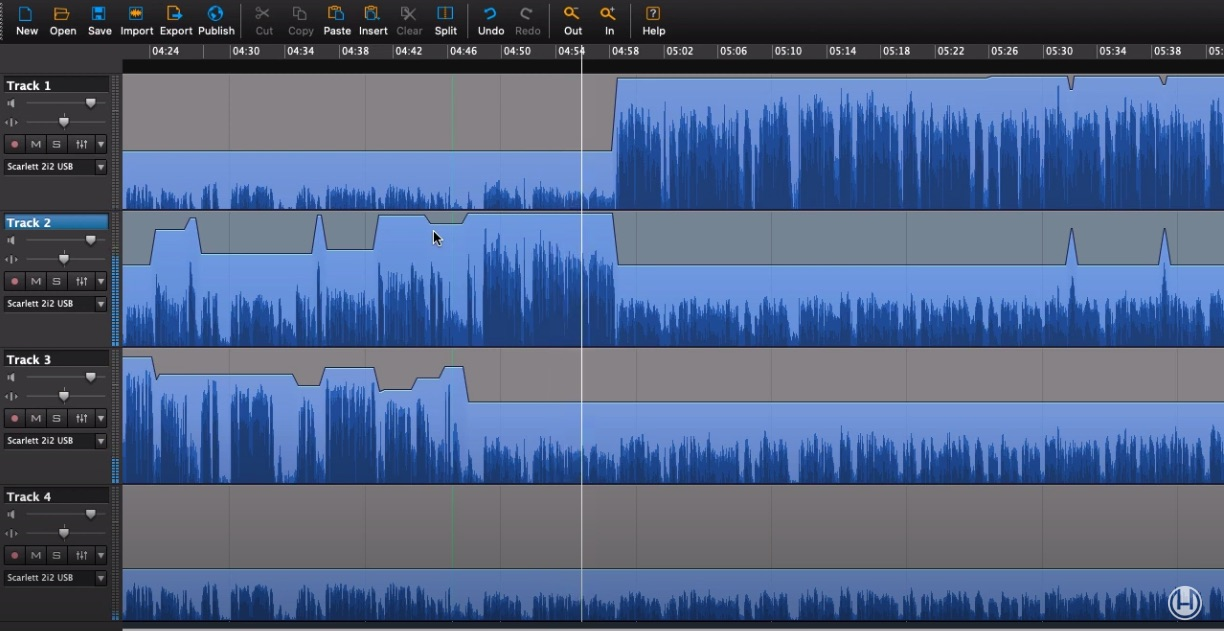
\includegraphics{images/hindenburg.jpg} Hindenburg Pro juga merupakan
software editing audio yang ditargetkan kepada podcaster dan jurnalis.
Software ini lintas platform dan bekerja dengan Windows dan macOS.
Hindenburg Pro juga dapat mengimpor file audio 24-bit dan bahkan bekerja
dalam sesi 24-bit. Selain itu, DAW membawa sejumlah besar efek termasuk
kompresor, EQ, loudness meters, dan dukungan untuk plugin vST sehingga
dapat memperluas pilihan efek yang diinginkan user.

Hindenburg memiliki fitur-fitur andalan seperti EQ otomatis, volume
normalization, de-bleed, dll yang tidak dimiliki oleh aplikasi
kompetitor lainnya. Alur kerja Hindenburg ramping dan intuitif. Dapat
mengimpor audio dari proyek lain, seperti audio dari perekam suara, atau
dapat merekam langsung ke dalam software ini sendiri.
